%!TEX program = lualatex
\documentclass[border=0mm,11pt]{standalone}
%\usepackage{color}
%\usepackage{tikz}
\usepackage[T1]{fontenc}
\usepackage[sc]{mathpazo}
\usepackage{tikz-feynman}
\usepackage{amsmath}
\tikzfeynmanset{compat=1.1.0}


\begin{document}

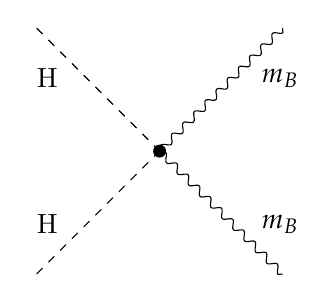
\begin{tikzpicture}[]
    \begin{feynman}
    \vertex (a);
    \vertex [below right=of a, xshift=0.5cm, yshift=-0.5cm] (cent);
    \vertex [above right=of cent, xshift=0.5cm, yshift=0.5cm] (b);
    \vertex [below left =of cent, xshift=-0.5cm, yshift=-0.5cm] (c);
    \vertex [below right =of cent, xshift=0.5cm, yshift=-0.5cm] (d);
    \node [dot] at (cent) {};
    \diagram* {
    (a) -- [scalar, edge label'=\(\text{H}\), near start] (cent) -- [boson, edge label'=\(m_{B}\), near end] (b),
    (c) -- [scalar, edge label=\(\text{H}\), near start] (cent) -- [boson, edge label=\(m_{B}\), near end] (d),
    };
    \end{feynman}
\end{tikzpicture}

\end{document}